\IfFileExists{revtex4-1.cls}{\documentclass[prd, twocolumn, lengthcheck,
superscriptaddress, showpacs, letterpaper, nofootinbib]{revtex4-1}}{ 
\IfFileExists{revtex4.cls}{\documentclass[prd, preprint,
superscriptaddress, showpacs, letterpaper, nofootinbib]{revtex4}}{}
}


\usepackage{amsmath}
\usepackage{hyperref}
\usepackage{color}
\usepackage{graphicx}

\newcommand{\vtheta}{\vec{\theta}}

\newcommand{\be}{\begin{equation}}
\newcommand{\ee}{\end{equation}}
\newcommand{\bel}[1]{\begin{equation}\label{#1}}
\newcommand{\ba}{\begin{eqnarray}}
\newcommand{\ea}{\end{eqnarray}}
\newcommand{\bal}[1]{\begin{eqnarray}\label{#1}}

\newcommand{\ilya}[1]{{\color{red} \bf Ilya: #1}}
\newcommand{\will}[1]{{\color{blue} \bf Will: #1}}

\newcommand{\order}[1]{\mathcal{O}\left( #1 \right)}

\def\aj{Astronomical Journal}                 % Astronomical Journal
\def\apj{Astrophysical Journal}                % Astrophysical Journal
\def\apjl{Astrophysical Journal}             % Astrophysical Journal, Letters
\def\pasj{PASJ}
\def\apjs{ApJS}              % Astrophysical Journal, Supplement
\def\mnras{MNRAS}            % Monthly Notices of the RAS
\def\prd{Phys.~Rev.~D}       % Physical Review D
\def\prl{Phys.~Rev.~Lett}    % Physical Review Letters
\def\cqg{Class.~Quant.~Grav.~}%Classical and Quantum Gravity
\def\araa{ARA\&A}             % Annual Review of Astron and Astrophys
\def\nat{Nature}              % Nature
\def\aap{A\&A}                % Astronomy and Astrophysics

\IfFileExists{apsrev4-1.bst}{\bibliographystyle{apsrev4-1}}
\IfFileExists{apsrev4.bst}{\bibliographystyle{apsrev4}}

\begin{document}
\title{An Efficient Interpolation Technique for Jump Proposals in
  Reversible-Jump Markov Chain Monte Carlo Calculations}

\date{\today}

\author{Will M. Farr}
\email{w-farr@northwestern.edu}

\affiliation{Northwestern University Center for Interdisciplinary
  Research and Education in Astrophysics}

\author{Ilya Mandel}
\email{ilyamandel@chgk.info}

\affiliation{MIT Kavli Institute; and University of Birmingham, UK}

\begin{abstract}
  Selection among alternative theoretical models given an observed
  data set is an important challenge in many areas of physics and
  astronomy.
  %ranging from gravitational-wave data analysis to
  %measurements of black-hole masses in X-ray binaries.
  Reversible-jump Markov chain Monte Carlo (RJMCMC) is an extremely
  powerful technique for performing Bayesian model selection, but it
  suffers from a fundamental difficulty: it requires jumps between
  model parameter spaces, but cannot retain a memory of the favored
  locations in more than one parameter space at a time.  Thus, a naive
  jump between parameter spaces is unlikely to be accepted in the MCMC
  algorithm and convergence is correspondingly slow.  Here we
  demonstrate an interpolation technique that uses samples from
  single-model MCMCs to propose inter-model jumps from an
  approximation to the single-model posterior of the target parameter
  space.  The interpolation technique, based on a kD-tree data
  structure, is adaptive and efficient in arbitrary dimensions.  We
  show that our technique leads to dramatically improved convergence
  over naive jumps in an RJMCMC, and compare it to other proposals in
  the literature to improve the convergence of RJMCMCs.  We also
  discuss the use of the same interpolation technique in two other
  contexts: as a convergence test for a single-model MCMC and as a way
  to construct efficient ``global'' proposal distributions for
  single-model MCMCs without prior knowledge of the structure of the
  posterior distribution.
\end{abstract}

\maketitle

\section{Introduction}

Selection among alternative theoretical models given an observed data
set is an important challenge in many areas of physics and astronomy.
In a Bayesian context, model selection involves computing the evidence
for each model given the data.  The model evidence is an integral of
the unnormalized posterior probability distribution over the model
parameter space, representing the probability of obtaining the data set within that model.
Models with larger evidence are preferred; the ratio of the evidences
of two models is the Bayes factor between them.  The product of the
Bayes factor and the ratio of prior probabilities for the two models yields
the odds ratio for the models.

There are many ways to compute model evidences.  In low-dimensional
parameter spaces, the unnormalized posterior probability can be
evaluated on a grid or lattice and the integral can be performed
directly.  For many problems or models of interest, however, the
dimensionality of parameter space is too large to make this approach
practical, and stochastic sampling must be used.  

Markov Chain Monte Carlo (MCMC) methods attempt to stochastically
produce parameter samples with density proportional to the posterior
probability distribution.  In MCMC techniques, the primary target is
an accurate estimate of the posterior distribution.  (We note that an
alternative stochastic method for exploring a model parameter space,
nested sampling \cite{Skilling:2004, Skilling:2006,Feroz:2009},
focuses on evidence computation rather than sampling the posterior
probability density functions.)  It is not straightforward to compute
the model evidence from MCMC samples.  The most direct way to estimate
the evidence for a model from MCMC samples is to compute the
harmonic-mean estimator, but this estimator of the evidence suffers
from infinite
variance\cite{NewtonRaftery:1994,Chib:1995,vanHaasteren:2009}.  MCMC
implementations with parallel tempering \cite{EarlDeem:2005} allow for
evidence computation via thermodynamic integration, but these can be
computationally costly.

Reference \cite{Weinberg2009} gives a method for directly computing
the evidence integral from existing MCMC samples by using a kD-tree
data structure to decompose a parameter space into boxes containing
the MCMC sample points.  The integral is approximated as a sum over
box volumes.  This method is promising, but it is not clear in general
what statistical and systematic errors it introduces and how these are
affected by the shape of the posterior distribution from which the
MCMC samples.

When the goal is model selection between several known models, only
the \emph{relative} evidence of each model is needed.  In this
circumstance, the Reversible Jump MCMC technique first introduced in
Reference \cite{Green1995} is one of the most reliable and accurate
ways to compare the models.  Reversible Jump MCMC (RJMCMC), described
more fully in Section \ref{sec:reversible-jump}, performs a standard
MCMC in a superspace that is a direct sum of all the model parameter
spaces.  Such an MCMC involves both intra- and inter-model jumps; the
number of MCMC samples in each model's parameter space is proportional
to that model's relative evidence in the suite of models being
compared.

Implemented naively, RJMCMC has a significant drawback: because the
chain of samples must be Markovian, only the current sample is
available to the algorithm as it is choosing the next sample.  Each
time an RJMCMC transitions between models, the information about the
choices of parameter values in the previous model is lost; subsequent
jumps into that model must ``start fresh,'' and are correspondingly
unlikely to be accepted, delaying convergence of the RJMCMC sample
chain.

Here we introduce a technique for improving the acceptance ratio of
inter-model jumps in an RJMCMC, leading to dramatically improved
convergence of RJMCMC sample chains.  The technique uses a kD-tree
data structure to construct an approximation to each model's posterior
parameter distribution.  We draw jump proposals into the model from this approximation to its posterior.  Because jumps are proposed
preferentially to locations favored by the single-model posterior, the
RJMCMC compares ``good'' locations in parameter space across all the
models, and convergence is generally rapid.  We have successfully applied this RJMCMC technique to a 10-way model selection among alternative mass distribution models for black-hole X-ray binaries \cite{Farr2010}.

Reference \cite{Littenberg2009} proposed an alternate method for
producing inter-model jumps in an RJMCMC that relies on a box
decomposition of parameter space, but uses fixed-sized boxes.  The box
size is fixed, so the method cannot adapt to the local structure of
the posterior, and becomes asymptotically inefficient for
high-dimensional parameter spaces or highly peaked posteriors.
Meanwhile, the approximation to the posterior distribution produced by
the kD-tree is a constant-in-box interpolation of the posterior,
similar in spirit to the phase-space density interpolants produced
from N-body positions and momenta in Reference \cite{Ascasibar2005}.
The kD-tree interpolation is effective in parameter spaces of
arbitrary dimensionality, and is quite space-efficient, requiring
$\order{N}$ storage space and $\order{\log N}$ time to produce each
proposed jump, where $N$ is the number of single-model MCMC samples
used to construct the interpolation.


The structure of this paper is as follows.  In Section
\ref{sec:reversible-jump} we introduce in more detail the concept of a
Reversible Jump MCMC, and describe the fundamental difficulty with a
naive jump proposal in an RJMCMC.  In Section \ref{sec:kDTree} we
introduce the kD-tree data structure used to decompose the parameter space
into boxes for interpolation.  In Section \ref{sec:efficiency} we
demonstrate the efficiency gains that are achieved from use of the
interpolated jump proposal.  In Section \ref{sec:examples} we give
examples of some other uses of the interpolated jump proposal, and suggest its utility in the context of a
single-model MCMC.  Finally, in Section \ref{sec:conclusion}
we offer a summary and some concluding remarks on the method.

\section{Reversible Jump MCMC}
\label{sec:reversible-jump}

Reversible jump Markov chain Monte Carlo (RJMCMC) \cite{Green1995} is
a technique for Bayesian model comparison.  Below, we give a very
brief introduction to Bayesian analysis, describe a standard MCMC, and
introduce RJMCMC.

\subsection{Bayesian analysis}

Consider an observed data set $d$ and a set of competing models for
the data, indexed by an integer $i$: $\{M_i | i = 1, 2, \ldots \}$.
Each model has some continuous parameters, $\vtheta_i$; given the
model and its parameters, we can make a prediction about the
likelihood of observing the experimental data: $L(d|\vtheta_i, M_i)$.
Within the framework of each model, Bayes' rule gives us a way to
compute the posterior probability distribution function (PDF) for the
model parameters implied by the data:
\be
  p(\vtheta_i | d, M_i) = \frac{L(d|\vtheta_i, M_i) p(\vtheta_i|M_i)}{p(d|M_i)},
\ee
where $p(\vtheta_i |d, M_i)$ is the posterior distribution for the
model parameters $\vtheta_i$ implied by the data in the context of
model $M_i$, $p(\vtheta_i|M_i)$ is the prior probability of the model
parameters that represents our beliefs before accumulating any of the
data $d$, and $p(d|M_i)$, called the evidence, is an overall
normalizing constant that ensures that $p(\vtheta_i|d,M_i)$ is
properly normalized as a probability distribution on the $\vtheta_i$.
This implies that the evidence is equal to
\bel{evidence}
  p(d|M_i) = \int_{V_i} d\vtheta_i L(d|\vtheta_i, M_i) p(\vtheta_i|M_i),
\ee
where $V_i$ is the parameter space volume in model $M_i$.  For model
comparison, we are interested in the posterior probability of a
particular model, $M_i$, given the data, $p(M_i|d)$.  Using Bayes'
rule, we see that this involves the evidence (Eq.~\eqref{evidence}):
\be
p(M_i|d) = \frac{p(d|M_i) p(M_i)}{p(d)},
\ee
where $p(M_i)$ is our a priori belief in model $M_i$ and $p(d)$ is a
normalizing constant,
\be
p(d)=\sum_i p(d|M_i) p(M_i).
\ee

When selecting among alternative models, we are interested in finding
the model with the highest posterior probability $p(M_i|d)$.  However,
attempts to directly compute the evidence by performing the
integration in Eq.~\eqref{evidence} are generally very difficult in a
multi-dimensional, multi-modal parameter space when the likelihood has
to be evaluated numerically.  In particular, a grid-based integral
quickly becomes computationally unfeasible as the dimensionality of
$\vtheta$ exceeds a few.  The parameter space must typically be
explored in a stochastic manner before the evidence integral can be
computed.  There are several stochastic parameter-exploration
techniques focused directly on evidence computation (e.g., nested
sampling \cite{Skilling:2004,Skilling:2006} and its variant MultiNest
\cite{Feroz:2009}).  Although nested sampling can be used to compute
the posterior PDFs within each model along with the evidences for the
various models, the most common technique for computing posterior PDFs
in the context of a model is the Markov chain Monte Carlo, which we
now describe.

\subsection{Markov chain Monte Carlo} \label{sec:mcmc}

A Markov chain Monte Carlo \cite{Gilks:1996} produces a set of samples
$\{ \vtheta^{(j)} \, | \, i = 1, \ldots \}$ from the model parameter
space that are sampled according to the posterior, meaning that, in
the limit that the chain length tends to infinity, the relative
frequency with which a given set of parameter appears in the chain is
proportional to the desired posterior, $p(\vtheta|d,M)$.  Therefore,
the output of an MCMC can be directly interpreted as the posterior PDF
over the full parameter space, while PDFs for individual parameters
can be obtained by marginalizing over the uninteresting parameters.

A Markov chain has the property that the probability distribution of
the next state can depend only on the current state, not on the past
history: 
%
\be 
p(\vtheta^{(j+1)})=\int_{V} d\vtheta^{(j)} p(\vtheta^{(j)} \to
\vtheta^{(j+1)}) p(\vtheta^{(j)}), \ee
%
where the jump probability $p(\vtheta^{(j)} \to \vtheta^{(j+1)})$
depends only on $\vtheta^{(j)}$ and $\vtheta^{(j+1)}$.  An additional
requirement for an MCMC arises from the fact that the desired
distribution is the equilibrium distribution.  In other words, if we
assume that state $(j)$ of the chain is sampled from the desired PDF,
$p(\vtheta^{(j)})=p(\vtheta^{(j)}|d,M)$ , then the next state $(j+1)$ must
be sampled from the PDF as well, so that
$p(\vtheta^{(j+1)})=p(\vtheta^{(j+1)}|d,M)$; this condition is known as
``detailed balance.''

One way to produce such a sequence of samples is via the
Metropolis-Hastings algorithm, first proposed in Reference
\cite{Metropolis:1953}, and later generalized by Hastings \cite{Hastings:1970}:
\begin{enumerate}
\item Given a current state $\vtheta^{(j)}$, propose the next state
  $\vtheta^p$ by drawing from a jump proposal distribution with
  probability $Q(\vtheta^{(j)} \to \vtheta^p)$.
\item Compute the probability of accepting the proposed jump as
  \bel{eq:p-accept} 
p_{\textnormal{accept}} \equiv \min\Bigl(1,
\frac{p(\vtheta^p|d)}{p(\vtheta^{(j)}|d)} \frac{Q(\vtheta^p \to
  \vtheta^{(j)})}{Q(\vtheta^{(j)} \to \vtheta^p)} \Bigr).  
\ee
\item Pick a uniform random number $\alpha \in [0,1]$.  If $\alpha<
  p_{\textnormal{accept}}$, accept the proposed jump, setting
  $\vtheta^{(j+1)}=\vtheta^p$.  Otherwise, reject the jump, and remain
  at the same location in parameter space for the next step,
  $\vtheta^{(j+1)}=\vtheta^{(j)}$.
\end{enumerate}
 
This jump proposal distribution $Q(\vtheta^{(j)} \to \vtheta^p)$ can
depend on the parameters of the current state $\vtheta^{(j)}$, but not
on the past history.  It must also allow any state within the prior
volume to be reachable (eventually) by the MCMC.  Any jump proposal
that satisfies these properties is suitable for an MCMC.

The jump proposal is the most important choice in the MCMC, as it
determines the sampling efficiency of the algorithm, i.e., the length
of the chain before it converges to the posterior PDF.  Creating an
efficient jump proposal distribution requires an understanding of the
structure of the parameter space which may not be available until the
PDFs are found, creating a Catch-22; one possibility for resolving
this infinite loop is described in Section \ref{sec:examples}.

It should be noted that although an MCMC whose jump acceptance
criterium obeys detailed balance (as the Metropolis-Hastings algorithm
does) must eventually converge to the desired distribution, there is
no way to guarantee convergence in a fixed number of steps or to test
whether a chain has converged in a foolproof manner.  For example,
MCMC chains can get stuck on local maxima, producing an apparently
well-converged sampling of the PDF in the vicinity of the maximum; or,
if the chain visits a sequence of local maxima, moving rarely between
maxima, the autocorrelation length of the chain may represent a
substantial fraction of the total number of samples, resulting in an
effective sample size that is too small to accurately represent the
relative sizes of the modes in the PDF (however, see Section
\ref{sec:examples} for one intriguing suggestion for remedying this
issue).

Finally, we note that, in practice, the randomly chosen initial
starting point of the MCMC may be in a particularly unlikely location
in the parameter space.  Because jumps are frequently local, we will
generally want to ignore the early points in a finite-size chain to
avoid biases in the recovered posterior PDF due to the choice of the
initial location.  The points thus discarded are referred to as
``burn-in'' points.

\subsection{RJMCMC}

The samples produced by an MCMC algorithm can be used to directly
perform a Monte Carlo evidence integral.  This results in a harmonic
mean estimator for the evidence, which suffers from a large variance
and bias \cite{NewtonRaftery:1994,Chib:1995,vanHaasteren:2009}.
Additional techniques for the direct integration of evidence, also
based on a kD tree decomposition of the parameter space (see
Sec.~\ref{sec:kDTree}), are described in \cite{Weinberg2009}.  These
techniques are promising, but in some cases suffer \cite{Farr2010}
from large variance and bias.  An alternative approach to model
selection among a set of models is based on performing an MCMC in a
``super-model'' that encompasses all of the models under
consideration; this is known the the Reversible Jump Markov chain
Monte Carlo (RJMCMC).

The parameter space of the super-model in an RJMCMC consists of a
discrete parameter that identifies the model, $M_i$, and a set of
continuous parameters appropriate for that model, $\vtheta_i$.  Thus,
each sample consists of a model identifier and a location within the
parameter space of that model, $\{M_i, \vtheta_i\}$.  We perform the
MCMC in the ``super-model'' parameter space just like a regular MCMC;
we propose jumps to different parameters within a model (intramodel
jumps) and jumps to a different model with different parameters
(intermodel jumps).  The resulting chain samples from the posterior
$p(M_i,\vtheta_i|d)$.  As in a usual MCMC, the PDF on the model as a
parameter, with other parameters ignored, is obtained by marginalizing
over the remaining parameters.  The posterior probability of a model
is proportional to the number of counts
%
\be
%
p(M_i|d) = \int d\vtheta_i \frac{p(d|M_i, \vtheta_i) p(M_i, \vtheta_i)}{p(d)}
\approx \frac{N_i}{N},
%
\ee
%
where $N_i$ is the number of RJMCMC samples listing the $i$'th model
and $N$ is the total chain length.  Thus, the probability of a
particular model relative to other models under consideration is given
by the fraction of RJMCMC samples lying in the parameter space of that
model.
 
The main difficulty of achieving an efficient RJMCMC is finding a good
jump proposal distribution for intermodel jumps.  In order to have
relatively high acceptance ratios for intermodel jumps, which is
necessary for efficient mixing between models, jumps should be
preferentially proposed into regions with a high posterior.  However,
because the algorithm is Markovian, it has no past memory, so a jump
proposed into a model from outside can not access information from
earlier in the chain which may identify a posterior peak.

The way to solve this problem is to identify a good jump proposal
distribution in advance, by exploiting information from single-model
MCMCs to generate efficient jump proposal distributions for our
reversible jump MCMC.  (Single-model MCMCs can take small local jumps
within their model, meaning that they are much less likely than an
RJMCMC to lose a high-posterior mode once it has been located.)  The
ideal jump proposal distribution for the parameters within a model
would consist of the posterior PDF for those parameters,
$p(\vtheta_i|M_i,d)$, and single-model MCMCs already represent samples
from these posterior PDFs.  However, the samples are discrete, and a
jump proposal must be continuous.  Therefore, the output of each
single-model MCMC must be interpolated to construct the desired jump
proposal.  The novel strategy we propose for efficiently interpolating
a discretely sampled PDF is described in the next section.

\section{kD Trees and Interpolation}
\label{sec:kDTree}

%\ilya{I think this section could just be phrased in terms of interpolation rather than jump proposal distributions; i.e., "the problem of finding the local density" instead of "the problem of drawing a proposed jump", etc.}

The problem of drawing a proposed jump from an interpolation of
single-model MCMC points can be thought of as the problem of assigning
a local ``neighborhood'' to each point in the chain of MCMC samples.
We choose these neighborhoods to be non-overlapping and fill parameter
space.  To draw a proposed jump, we select a point uniformly from the
MCMC samples, find its associated neighborhood, and then draw the
proposed jump uniformly from the neighborhood.  Since the MCMC points
are distributed according to the posterior PDF for the single model,
this procedure produces proposed jumps that are approximately
distributed according to the posterior PDF.  The size of a
neighborhood is inversely proportional to the local point density.
The proposed jumps are drawn from a piecewise-constant (constant on
each neighborhood) interpolation of the PDF.  There are various
techniques that could be used to construct the set of neighborhoods
associated with each point.

Ref.~\cite{Littenberg2009} decomposed the parameter space into
constant-volume ``bricks'' whose size was set by the typical size of
the peaks of the PDF.  Each sample was associated with the brick that
contained it, and the probability of proposing a jump into a particular brick is thus proportional to the
number of samples within that brick.  Additionally, an extra uniform jump proposal was added to allow for jumps into bricks that did not contain any points, so that the jump 
proposal covers the entire model parameter space.  
However, the bricks in this algorithm do not adapt to the local
structure of the PDF.  One must either use small bricks to capture the
local structure of the PDF, placing many bricks in regions without
MCMC samples (which can increase memory management and access costs),
or use large bricks, missing the local structure of the PDF in
exchange for fewer empty bricks.

An alternate technique for producing adaptive neighborhoods would be
to use the Voronoi regions \cite{Voronoi1907} associated with each
MCMC sample.  The Voronoi region associated with a sample contains all
the parameter space points that are closer to that sample than any
other sample.  The Voronoi region decomposition into neighborhoods is,
in a sense, maximally adaptive, in contrast to the approach of
Ref.~\cite{Littenberg2009}, which is minimally adaptive.
Unfortunately, defining the Voronoi regions requires a metric on
parameter space, which may be difficult or impossible to define.
Also, the computational cost for computing the Voronoi regions
increases rapidly with dimensionality.  
% Apparently the exact computational cost is not known in arbitrary dimension.

Here we propose to use a decomposition of the parameter space into
neighborhoods based on a data structure called a kD-tree (see, e.g.\
\cite{Berg2008} or \cite{Gaede1998}).  The decomposition is more
adaptive than the cells of Ref.~\cite{Littenberg2009}, and more
efficient in high-dimensional spaces than the Voronoi decomposition.

A kD-tree is a binary, space-partitioning tree.  To partition a set of
points into a kD-tree, begin by placing them in a rectangular box that
contains all of parameter space.  Then proceed recursively:
\begin{enumerate}
\item If the given box contains exactly one point, stop; this is a
  leaf of the tree.  Otherwise:
\item Choose a dimension along which to divide the points.  Divide the
  points in half along this dimension (or nearly in half, if the
  number of points is odd), forming two sub-boxes.  The ``left''
  sub-box contains the half (or nearly half) of the points that have
  small coordinates along the chosen dimension; the ``right'' sub-box
  contains the half (or nearly half) of the points that have large
  coordinates along the chosen dimension.
\item Return to Step 1 with each of the sub-boxes, storing the
  resulting trees as sub-trees of the current box.
\end{enumerate}
The key algorithmic step in the production of a kD-tree is finding the
median point along a given dimension in order to divide the points in
half in Step 2.  For $n$ points, this can be accomplished in
$\order{n}$ time (see, e.g., Ref.~\cite{Press2007}).  If there are $N$
points in total, there are $\order{\log N}$ levels in the tree; at
each level, $\order{N}$ points must be processed once in the
median-finding algorithm.  Tree construction thus costs $\order{N \log
  N}$ in time, and the tree consumes $\order{N}$ space.  As an
illustration, box boundaries for a kD-tree constructed around a point
set that is normally distributed around the origin in two dimensions
are shown in Figure \ref{fig:kD-tree}.

\begin{figure}
  \begin{center}
    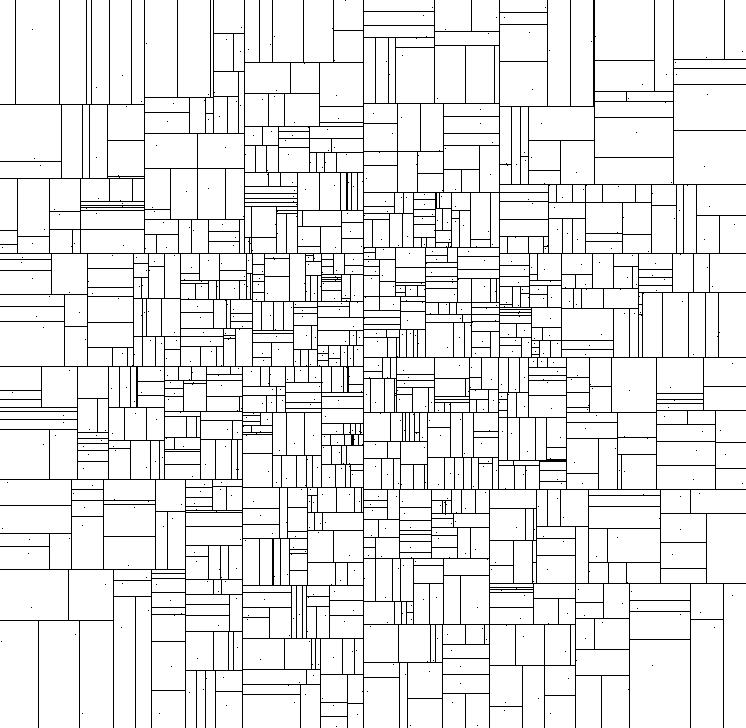
\includegraphics[width=0.8\columnwidth]{kdtree.png}
  \end{center}
  \caption{\label{fig:kD-tree} The neighborhoods from a kD-tree
    constructed around a set of points that are normally distributed
    about the origin in two dimensions.  As the points become denser
    around the origin, the typical neighborhood gets smaller.  The
    interpolated PDF within a box of volume $V_i$ is $1/(N V_i)$,
    where $N$ is the total number of points (which is also the number
    of boxes).}
\end{figure}

In order to use the kD-tree interpolation as a jump proposal in an
MCMC, we must be able to quickly find the neighborhood associated with
a given point to compute the jump probability (see
Eq.~\ref{eq:p-accept}).  This can be accomplished in $\order{\log N}$
time and constant space with the following algorithm, which is a
standard binary tree search.  Given the point, $\vtheta_i$ and the
tree, $T$:
\begin{enumerate}
\item If $T$ contains exactly one sample point, then its box is the
  associated neighborhood.  Otherwise:
\item The tree $T$ has two sub-trees.  If the point $\vtheta_i$ is
  contained in the ``left'' sub-tree, then return to Step 1,
  considering this sub-tree; otherwise return to Step 1, considering
  the ``right'' sub-tree.
\end{enumerate}

\section{RJMCMC Efficiency}
\label{sec:efficiency}

In this section, we demonstrate the efficiency of the kD-interpolated
jump proposal on a toy model-comparison problem.  We draw $N = 100$
simulated data points from a $N(0,1)$ Gaussian distribution, and then
ask whether these data are better described by a model where they are
Gaussian distributed with unknown mean $\mu$ and standard deviation
$\sigma$
%
\be
p(x) = \frac{1}{\sqrt{2\pi} \sigma} \exp\left( - \frac{(x-\mu)^2}{2
    \sigma^2} \right)\ ,
\ee
%
or by a model where they are Cauchy distributed with mode $\alpha$
and width $\beta$
%
\be
p(x) = \frac{1}{\pi \beta \left( 1 + \left(\frac{x - \alpha}{\beta}\right)^2\right)}\ .
\ee
%
We take priors on $\mu$ and $\alpha$ to be uniform in $[-1,1]$, and
priors in $\sigma$ and $\beta$ to be uniform in $[0.5, 1.5]$.  With a
data set of 100 points, the relative uncertainty in determining the
parameters of the underlying distribution is approximately 10\%, so we
expect the posterior probabilities in the $(\mu,\sigma)$ and
$(\alpha,\beta)$ spaces to occupy only a few percent of the prior
volume.  The Cauchy distribution is much broader than the Gaussian (it
has no finite moments), so with uniform model priors, the posterior
probability for the Gaussian model over the Cauchy model is extremely
large:
%
\be
\frac{p(\textnormal{Gaussian} | d)}{p(\textnormal{Cauchy}|d)} \sim 10^9.
\ee
%
In order to ensure that the RJMCMC produces samples in the Cauchy
model at all, we impose a model prior that favors the Cauchy model by
$5 \times 10^8$ relative to the Gaussian.  The evidence ratio between
the models for our chosen data set with these priors is
%
\be \frac{p(\textnormal{Gaussian} | d)}{p(\textnormal{Cauchy}|d)}
\equiv r = 1.15,
\ee
%
yielding a theoretical maximum acceptance rate of inter-model jumps of
$(1+1/r)/2 = 0.93$.

We obtain $10^4$ single-model MCMC samples by independently running MCMC within each model, and use the kD-tree interpolation method described above to propose
inter-model jumps in an RJMCMC.  The acceptance rate of inter-model
jumps is approximately 0.8.  To explore how the efficiency of the
method degrades as the interpolation becomes less accurate, we
artificially truncated the kD tree with higher and higher numbers of
points in each box (this can be accomplished during the neighborhood
search phase by stopping the search for a box when one is found
containing the desired number of points).  For each truncation choice, we
performed an RJMCMC with the resulting interpolated jump proposal.
The acceptance rate is plotted against the number of single-model MCMC points per box (kD-tree leaf) in Figure \ref{fig:acceptRate}.  The more points in each leaf of the tree when
the search is truncated, the lower the acceptance probability; when
points are drawn from the top level of the tree, the acceptance
probability asymptotes to the naive draw from the prior ($\sim 5\%$).

\begin{figure}
  \begin{center}
    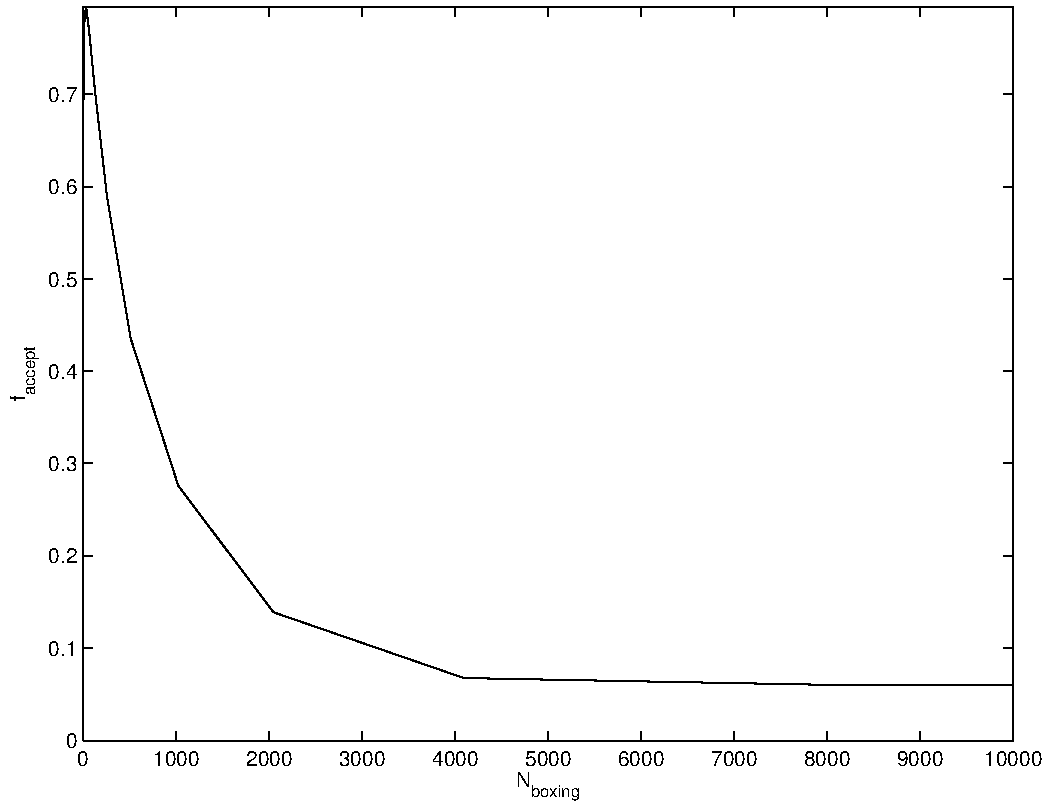
\includegraphics[width=0.8\columnwidth]{acceptRate}
  \end{center}
  \caption{\label{fig:acceptRate} The inter-model acceptance rate
    versus the number of points per box when the kD-tree neighborhood
    search is truncated.  As the number of points per box increases,
    and the interpolation becomes less accurate, the acceptance rate
    falls, asymptoting to the rate for naive draws from the uniform
    prior (about $5\%$ for this data set).}
\end{figure}

The relative error on the determination of the Bayes factor (evidence ratio) scales
with $1/\sqrt{N_{\textnormal{transitions}}}$, where
$N_{\textnormal{transitions}}$ is the number of inter-model
transitions in the RJMCMC.  Thus, as the acceptance rate of
inter-model jumps goes down, the RJMCMC must run longer to achieve a
desired accuracy in the evidence ratio.  By boosting the acceptance
rate of inter-model jumps, the interpolation method described above
can dramatically improve the runtime of an RJMCMC.

\section{Examples and other uses} 
\label{sec:examples}

RJMCMC with efficient PDF interpolation via kD trees can be used in a large variety of problems in physics and astronomy, whenever Bayesian analysis is used to perform model selection.  Below, we describe several scenarios in which we have successfully applied this technique.  Moreover, PDF interpolation with a kD tree can be extremely useful in other contexts, beyond a reversible-jump MCMC.  We suggest two examples below: generating efficient jump proposal distributions in a single-model MCMC and convergence tests.


We have successfully employed the RJMCMC technique described above
when evaluating several alternative models for the distribution of the
masses of black holes in X-ray binaries \cite{Farr2010}.  We
performed a Bayesian analysis of the mass distribution of stellar-mass
black holes using the observed masses of 15 low-mass X-ray binary
systems undergoing Roche lobe overflow and five high-mass, wind-fed
X-ray binary systems.  We considered ten different mass distribution
models: Gaussian, double Gaussian, power law, exponential decay, log
normal, and 1-, 2-, 3-, 4-, and 5-bin histograms.  Each model was
described by between two and six parameters.  Model selection using
RJMCMC with kD trees allowed us to determine that the mass
distribution of the low-mass systems is best fit by a power-law, while
the distribution of the combined sample is best fit by the exponential
model.  Based on the model selection, we were able to determine which
models would provide the best information about astrophysically
relevant parameters, such as the minimum black hole mass.  We were
also able to conclude that the low-mass subsample is not consistent
with being drawn from the distribution of the combined population
\cite{Farr2010}.

Gravitational-wave astronomy provides the setting for another ongoing
study.  Interesting triggers from the LIGO \cite{InitLIGO} and Virgo \cite{Virgo}
gravitational-wave detector pipeline that searches for compact binary
coalescences are followed up with Bayesian parameter estimation tools (see, e.g., \cite{Rover:2006ni, vanderSluys:2008b, VeitchVecchio:2009}).
In general, several possible models for the data are considered,
including a pure noise model, noise superimposed on a non-spinning
gravitational-wave signal, or noise superimposed on a gravitational
wave signal that includes significant spin or spins in the binary
components.  The models can include a large number of parameters (up
to 15 for the model with two spinning components \cite{Raymond:2010}), and RJMCMC with
interpolation via kD trees is again successful at computing the model
evidences. 

As discussed in Section \ref{sec:mcmc}, finding an efficient jump
proposal distribution can be a challenge even for a single-model MCMC.
This is particularly difficult when the parameter space is
multi-modal, in which case the Markov chain can get stuck on
individual high-posterior islands in the parameter space.  Traversals
of low-posterior oceans by a series of short jumps are extremely
unlikely, and random long jumps are almost always rejected, making
sampling very inefficient.  Essentially, such isolated islands in
parameter space behave as separate models, and weighting them by the
number of samples in each peak then corresponds to model selection.
Ideally, an analytical understanding of the model would allow for the
creation of jump proposal distributions that combine short jumps
designed to explore individual islands with directed long jumps that
are likely to end up on neighboring islands.  However, it is not
always possible to gain such understanding short of performing the
MCMC itself.  One solution lies in running multiple chains that
explore the parameter space, perhaps getting stuck on local maxima,
and then combining the points and interpolating with a kD tree to
create a jump proposal distribution.  Although the chains in the first
iteration will not have transitioned between the peaks, and the
samples will therefore not weight the separate peaks appropriately,
this will ensure that all of the modes (islands) are included in the
jump proposal distribution for a second stage.  This second stage can
employ an interpolated jump proposal exactly as in the model selection
discussed above.  Other modifications to this technique, which we are
currently investigating, include multiple iterative stages, with the
interpolated samples from each previous stage used as a jump proposal
distribution for the next stage, until the posterior PDF is read off
from the final stage; and the use of higher temperatures in the
early-stage chains to improve sampling.

An example of a multi-modal parameter space where chains can get stuck
on high-posterior islands comes from antipodal sky location
degeneracies for networks of three ground-based gravitational-wave
interferometers or for low-frequency gravitational wave signals in the
proposed space-borne instrument LISA \cite{LISA}.  Although PDFs
produced by MCMC chains will generally show both locations on the sky,
the chain length may not be sufficiently long in practice to include
enough jumps between the two high-likelihood antipodal locations.  In
general, the relative weight of two separated peaks is determined with
a fractional error that scales as
$1/\sqrt{N_{\textnormal{transitions}}}$, where
$N_{\textnormal{transitions}}$ is the number of transitions between
the peaks.  By increasing the number of proposed transitions, the
convergence of such PDFs can be enhanced using the kD tree
interpolated proposal.  

\section{Conclusion}
\label{sec:conclusion}

The need to compare evidences for multiple models arises in a large variety of physical and astronomical contexts.  In this paper, we described a new technique that allows for efficient evidence computations via a Reversible-Jump Markov chain Monte Carlo.  This technique solves the usual problem of finding good inter-model jump proposals in an RJMCMC by using a kD-tree to quickly and accurately interpolate an approximate posterior PDF from a single-model MCMC run, and then using this interpolated PDF to propose efficient inter-model jumps.  

We demonstrated the efficiency of this technique on a toy model-comparison problem described in Section \ref{sec:efficiency}.  We also successfully applied this technique to the problem of selecting the best model for the observed distribution of black-hole X-ray binaries, as described in Section \ref{sec:examples} and Ref.~\cite{Farr2010}.   In addition to model comparison, the PDF interpolation described here can be useful in multi-step MCMCs to improve the sampling efficiency by selecting better jump proposal distributions or to test MCMC convergence.

We have made our implementation of the technique described in this paper publicly available online at \will{URL}, and welcome readers to take advantage of this toolkit.


\section*{Acknowledgments}

We are grateful to Neil Cornish for interesting discussions.  IM acknowledges support from the NSF Astronomy and Astrophysics Postdoctoral Fellowship, award AST-0901985.  WF acknowledges support from \will{Add your acknowledgements}

\bibliography{paper}

\end{document}
